
\documentclass[12pt]{article}

% graphics 

\makeatletter
\@ifpackageloaded{tex4ht}{%
\usepackage[dvipdfmx]{xcolor}
\usepackage[dvipdfmx]{graphicx}
\usepackage[tex4ht]{hyperref}
}{%
\usepackage{xcolor}  % [pdftex] explicit specification works for pdflatex only 
\usepackage{graphicx}% [pdftex] explicit specification works for pdflatex only 
\usepackage{hyperref}% driver [hpdftex] is autodetected 
}

\usepackage{svg}

% synchronization between tex and pdf 
\usepackage[active]{srcltx}


\usepackage{longtable}
\usepackage{listings}
\usepackage{fancyvrb}

% only with pdflatex, warnings for xelatex and for lualatex 
% ifxetex, ifluatex, ifpdf
\usepackage{ifpdf,ifxetex,ifluatex}
\ifpdf
%\usepackage[utf8]{inputenc}
\usepackage[T1]{fontenc}
\else
\fi

% index and glossary
\usepackage{makeidx}
\makeindex
\usepackage[toc, xindy]{glossaries}
%, xindy or even [xindy={language=english,codepage=utf8}]

\makeglossaries

\setacronymstyle{long-short}
% file formats 
\newacronym{pdf}{pdf}{portable document format}
\newacronym{dvi}{dvi}{device independent file format}
\newacronym{eps}{eps}{encapsulated postscript}
\newacronym{tex}{tex}{tex the format, which may also be latex}
\newacronym{html}{html}{hypertext markup language}
\newacronym{xhtml}{xhtml}{extensible hypertext markup language}
\newacronym{odt}{odt}{open document text}
\newacronym{doc}{doc}{outdated document format for MS word }
\newacronym{docx}{docx}{current document format for MS word }
\newacronym{sgml}{sgml}{Standard generalized markup language }
\newacronym{xml}{xml}{extensible markup language }
\newacronym{ptx}{ptx}{pdf/postscript tex format }% home brewed 
% plt missing 
\newacronym{fig}{fig}{native file format for xfig }
\newacronym{png}{png}{Portable Network Graphics}
\newacronym{jpg}{jpg}{Graphics format developed by the Joint Photographic Experts Group }
\newacronym{gif}{gif}{Graphics Interchange Format, allows also animations }
\newacronym{svg}{svg}{Scalable Vector Graphics}
% latex file endings 
\newacronym{toc}{toc}{table of contents}
\newacronym{lof}{lof}{list of figures}
\newacronym{lot}{lot}{list of tables}
\newacronym{aux}{aux}{auxiliary file}
\newacronym{log}{log}{logging file (for LaTeX and mpost)}
\newacronym{idx}{idx}{index file containing unsorted and multiple index entries}
\newacronym{ind}{ind}{%
index file containing sorted, unified and formatted index entries}
\newacronym{glo}{glo}{%
glossary file containing unsorted and multiple glossary entries}
\newacronym{gls}{gls}{%
glossary file containing sorted, unified and formatted glossary entries}


\newacronym{mp}{mp}{metapost}
\newacronym{ps}{ps}{PostScript}
\newacronym{mps}{mps}{metapost's postscript like output including text}
\newacronym{mpx}{mpx}{metapost tex output: texts }

% \newglossaryentry{latex}{name={\latex},description={%
% A document preparation system 
% converting sources in the latex-format preferrably into pdf-output. 
% Historically, output was in \gls{dvi}-format 
% which is still used by htlatex as an intermediate format 
% to produce \gls{html} resp.~\gls{xhtml} and \gls{odt} output. 
% }}
% \newglossaryentry{htlatex}{name={htlatex},description={%
% A script which wraps latex 
% but producing (x)html and odt output instead of pdf 
% which is usual for latex. 
% }}
%\newglossaryentry{ps}{name={PostScript},description={%
%A computer language for creating vector graphics. 
%}}

\usepackage[nottoc, numindex, numbib]{tocbibind}

\title{Manual for the latex-maven-plugin and for an according ant-task }
\author{Ernst Reissner (rei3ner@arcor.de)}


\begin{document}
\maketitle

\tableofcontents
\listoffigures
\listoftables


\section{Introduction}

LaTeX is a beautyful way to create printable documents, 
today in preferrably as \gls{pdf}-files, 
with a particular strength in typesetting formulae like 
%
\begin{eqnarray*}
\pi & = & \sqrt{12}\;\sum^\infty_{k=0} \frac{(-3)^{-k}}{2k+1}. 
\end{eqnarray*}
%
Here, portability of the format \gls{pdf} is a vital feature. 

This piece of software implements both an ant-task and a maven-plugin 
generating documentation of various formats from LaTeX files 
in an uniform way. 
Besides \gls{pdf}, these formats include the web-formats \gls{html} 
and \gls{xhtml}, 
open offices format \gls{odt}, microsoft's word formats like \gls{docx} 
and finally plain text. 

Uniformity of ant-task and a maven-plugin means in particular, 
that the settings which may be passed to the task 
and those allowed for the plugin are in a one-to-one relation. 
They are both described in Section \ref{sec:settings}. 
\index{ant-task}
Both, the ant-task and the maven-plugin rely on the same code base 
which form the package {\tt org.m2latex.core}. 
The code specific for the ant-task is in {\tt org.m2latex.antTask} 
and that specific for the maven-plugin is in {\tt org.m2latex.mojo}. 

It is very usual to endow LaTeX-files with figures. 
We support figures created in the \gls{fig} by the program xfig, 
figures created by the plotting utility gnuplot, 
the tex-specific graphic language metapost 
and finally figures in formats which can be included into a latex-file 
without preprocessing like \gls{png} and \gls{jpg} 
or with automatic conversion like \gls{svg}. 
Further functionality on latex figures can be easily added. 
If there is some need, please write an email to the author. 

The creation process supports an index, a glossry and a bibliography. 
Again, further functionality can be added by demand. 

The present manual is created by the maven-pugin or the ant-task 
described here. 
There should be no difference in the result. 
This manual is designed in a way that it covers the most important features 
but also to demand the most important features. 
That way, creating this manual is a top level test 
for the underlying software. 
The maven-plugin is somehow superior 
because it better supports the design process for the latex sources. 



\section{Installation}

Both the ant-task and the maven-plugin just direct parameters 
from ant and from maven, respectively, 
to the programs that do the proper work. 
Thus installation of the ant-task and of the maven-plugin 
requires that all needed programs are installed. 
These prerequisites are collected in Section \ref{subsec:prerequisites}. 
\index{ant-task}

\subsection{Prerequisites}\label{subsec:prerequisites}

The ant-task is tested with 
{\tt Apache Ant(TM) version 1.9.4 compiled on September 11 2015}\index{ant}
and the maven-plugin with \index{maven}
%
\begin{verbatim}
Apache Maven 3.2.1
(ea8b2b07643dbb1b84b6d16e1f08391b666bc1e9; 
2014-02-14T18:37:52+01:00). 
\end{verbatim}
The java version is {\tt 1.8.0\_101, vendor: Oracle Corporation}. \index{java}

So, a java installation is the base for running either the ant-task 
or the maven-plugin. 
To use the maven-plugin, of course maven must be installed 
and to use the ant-task, ant must be installed. 

The ant-task just passes parameters in the build file to the core 
and accordingly the maven-plugin passes parameters in the pom 
to the core. 
The core just invokes various programs to do the actual work. 
\index{ant-task}

Depending on what kinds of graphic formats are used, 
the following programs are required: 
To convert the \gls{fig}-files into \gls{pdf}-files, 
by default {\tt fig2dev} is used. \index{fig2dev}
It makes sense to have {\tt xfig} installed \index{xfig}
to create and edit fig-files, but this is not mandatory. 
To convert gnuplot files into pdf-files, there is no alternative, 
to have installed {\tt gnuplot}. \index{gnuplot}
It serves as an interpreter and also as a converter. 
Strictly speaking, only the latter functionality is required here. 
To convert \gls{mp}-files into \gls{eps}-files, 
\index{mpost}\index{metapost}
the interpreter {\tt mpost} or equivalent is required. 
This comes with a standard tex-installation. 
To include \gls{svg}-files into latex \index{svg}, 
{\tt inkscape} must be installed. \index{inkscape}
It also serves to create and edit svg-files. 



Currently for including pdf-files in both cases, 
the driver {\tt dvipdfmx} must be installed. 
Strictly speaking, this is required only for html-creation and related. 
Note that if no pictures created by {\tt fig2dev}, {\tt gnuplot}, 
{\tt mpost} or by {\tt inkscape} are used, of course, 
neither {\tt fig2dev} nor {\tt gnuplot}, {\tt mpost}, {\tt inkscape} 
nor {\tt dvipdfmx} is needed. 
To include graphics, the grapics bundle described in \cite{GraX} is required, 
except for svg-files which requires the svg-package 
described in \cite{SvgP}. 

To create pdf-files from latex files we use {\tt pdflatex} 
or some other kind of latex creating pdf-files 
like {\tt xelatex} or {\tt lualatex}. 
\index{pdflatex}\index{xelatex}\index{lualatex} 
LaTeX uses several auxiliary programs. 
Above all {\tt bibtex} to create the bibliography 
and {\tt makeindex} for the index and {\tt makeglossaries} for the glossary. 
\index{bibtex}\index{makeindex}\index{makeglossaries}
The latter two 
also require the latex packages {\tt makeidx} and {\tt glossaries} 
described in \cite{MkidxShIdxP} and in \cite{GloP}. 
Note that {\tt makeglossaries} eiter invokes {\tt makeindex} 
or {\tt xindy}, depending on the parametrization of {\tt glossaries}. 
Both, {\tt makeglossaries} and {\tt xindy} are written in perl, 
which shall also be installed if a glossary is required. 

To create \gls{html}-files, 
or to be more precise any kind of \gls{sgml} and \gls{xml}, 
from latex-files, {\tt htlatex} or alternatively {\tt htxelatex} is used. 
Currently the author is not aware of any alternative to the two. 
This includes also creating open office documents like odt-files. 
Thus open office documents are created in two steps, 
the first is to create pdf-files with the according tools, 
the second one is done by {\tt htlatex} or that like. 
\index{htlatex}\index{htxelatex}

To create rtf-files, currently {\tt latex2rtf} is used. 
Note that this does not require {\tt pdflatex}. 
As a drawback, not all latex-packages are supported. 
\index{latex2rtf}

MS word documents are created from open office documents via {\tt odt2doc} 
and thus require three steps. 
\index{odt2doc} 

Finally, there is a way, to create plain text files from the pdf-files 
via {\tt pdftotext}. 
The way from latex to text via pdf makes sense 
because that text is well formatted 
and may contain unicode symbols like $\pi$. 
\index{pdftotext}

So to run this software, the abovementioned programs 
or at least the subset used, must be installed. 

\subsection{Setting pom.xml and build.xml}\label{subsec:sgml}

To install the maven-plugin within a given maven project, 
the listing of a pom entry given in Section \ref{sec:settings} 
can be added to {\tt pom.xml} and modified accordingly. 
In a default maven project, 
the default configuration is usable which creates pdf-documents and
\gls{html}-sites. 
The according entry to be added to the {\tt pom.xml} is then just 
%
\lstset{language=xml, basicstyle=\small}
\begin{lstlisting}
<!-- create html and pdf and other formats from latex -->
<plugin>
  <groupId>de.akquinet.jbosscc.latex</groupId>
  <artifactId>latex-maven-plugin</artifactId>
  <version>1.3-SNAPSHOT</version><!--uptodate?-->
  <!--artifactId>maven-latex-plugin</artifactId>
      <version>1.2</version--><!--uptodate?-->
</plugin>
\end{lstlisting}

Likewise to install the ant-task within an ant-project, 
the listing of a build file entry given in Section \ref{sec:settings} 
has to be added to the {\tt build.xml}. 
Also working with an ant project 
conforming with maven conventions, 
no explicit configuration is needed. 
\index{ant-task}

In both cases, add configuration, 
where a deviation from the default requires to do so. 



\subsection{Completing the Installation}\label{subsec:instComplete}

To install the maven-plugin, just type {\tt mvn clean install}. 
To install the ant-task, one has first to comment out in {\tt build.xml} 
the taskdef {\tt latex} and the target {\tt latex:cfg}. 
One may also adapt the lib-folder of the ant-installation, 
i.e. the property {\tt antJarDir} where {\tt ant.jar} resides. 
Then just type {\tt ant clean jar} 
which creates the jar-file (property {\tt createdJar}) defining the ant-task. 
After that one may copy the created jar into folder {\tt antJarDir}, 
where ant finds it typing {\tt sudo ant install}. 
\index{ant-task}

Note that, if maven is installed, the command {\tt mvn clean install} 
also creates the jar-file {\tt createdJar} defining the ant-task. 
Also with this method, one has to copy the jar-file defining the ant-task 
later into ant's lib-folder. 

After having installed the ant-task, 
reactivate the taskdef {\tt latex} and the target {\tt latex:cfg} 
and run {\tt ant latex:cfg} to create this manual. 

Mixing ant and maven builds is not so good. 
One may always recover by just creating with maven. 



\section{Usage of this Plugin and of this Task}\label{sec:usage}

This plugin may be used both if the latex-sources are finished 
to create the output described by them 
and also to support development of the latex sources. 
Accordingly, this section has two subsections. 

\subsection{The source files}\label{subsec:sources}

The latex-files and also files included via {\tt\textbackslash input} 
are in the {\em tex-source directory}, 
\index{tex-source directory}
which is by default {\tt./src/site/tex}, 
where {\tt.} is the {\em base directory} of this maven-project. 
\index{base directory}
The latex-files not included anywhere are called {\em latex main files}. 
\index{latex main file}
The included files may be again latex-files but also graphic files 
in various formats. 
There are three kinds of graphic formats, 
as regards the way their files are included in latex files. 
%
\begin{itemize}
\item
The first can be included into latex files directly 
via {\tt\textbackslash input}. 
These formats are essentially latex and are defined in an according package. 
An example is {\tt eepic} described in \cite{EEpic}. 
\item
the second one via {\tt\textbackslash includegraphics} 
defined by the package {\tt graphicx} 
which is described in \cite{GraX}. 
Chapter 2 therein mentions the supported drivers, 
among these also {\tt dvipdfm} and {\tt dvipdfmx}. 
It is not the package but the driver 
which decides on the support of graphic formats. 
The dvipdfm user manual, \cite{DviPdfMx} lists the allowed formats 
metapost-output (i.e. \gls{mps}), postscript, 
\gls{pdf}, \gls{jpg} and \gls{png}. 
\item
and the third one must be transformed into a graphics format 
of one of the former two kinds using an external tool for transformation. 
Here, of course, only a limited support is possible, 
because there is a broad variety of formats. 
We have choosen the \gls{fig}-format **** citation **** because of its simplicity, 
the gnuplot format, described in \cite{GnuPlot}, 
because it allows computation of pictures, 
likewise metapost, described in \cite{MPost}. 
\end{itemize}

The latex files and the graphic files belonging to a latex main file 
are assumed to be in one single folder. 
If one file is included by two different main files, 
a link shall be used. 


\subsection{Exporting in various formats}\label{sec:stableUsage}


After having added the configuration of the plugin to the {\tt pom.xml}, 
it can be used directly invoking maven through 
{\tt mvn latex:cfg}. 
Here {\tt latex} is the (short) name of the plugin and {\tt cfg} is the target. 
It can also be interpreted as {\tt mvn $<$source$>$:$<$target$>$}: 
The source files are in {\tt latex}-format and the target-format(s) 
are read from the {\em configuration} in the pom 
({\em configuration}h is what is what {\tt cfg} stands for). 
By default, the target formats are {\tt pdf} and {\tt html}. 
The following listing shows a configuration 
with the full range of output formats including in addition 
the open office document format {\tt odt}, 
the MS word-format(s) {\tt doc(x)} and {\tt rtf}
and also plain text format {\tt txt} in utf8 encoding. 
Note that the target {\tt docx} converts by default into \gls{docx} 
but may also be configured to produce the old fashioned \gls{doc} format. 
%
\lstset{language=xml, basicstyle=\small}
\begin{lstlisting}
<!-- create html and pdf and other formats from latex -->
<plugin>
  <groupId>de.akquinet.jbosscc.latex</groupId>
  <artifactId>latex-maven-plugin</artifactId>
  <version>1.3-SNAPSHOT</version><!--uptodate?-->
  <!--artifactId>maven-latex-plugin</artifactId>
      <version>1.2</version--><!--uptodate?-->
	
  <configuration>
    <settings>
      <targets>pdf, html, odt, docx, rtf, txt</targets>
    </settings>
  </configuration>
</plugin>
\end{lstlisting}

Sometimes it is more convenient 
to specify the output formats not via the pom 
but directly on the command line. 
In particular, one may write {\tt mvn latex:pdf} to create documentation 
in pdf-format only. 
Note that the {\tt -X} switch activates debugging 
which results in a more verbose output. 
Example: {\tt mvn -X latex:cfg}. 

There is another target for clearing the LaTeX {\em source} directory 
recursively, invoked by {\tt mvn latex:clr}. 
For more details on that see Section \ref{subsec:devel}. 

In a standard maven project, 
the above minimal configuration should be sufficient. 
Only if the folder structure deviates from the standard 
or if the latex sources require special configuation, 
parameters have to be given explicitly, 
because they deviate from the default values. 
Section \ref{subsec:settingsOverview} summarizes all available parameters, 
giving the default value and a description. 


For sake of uniformity, 
the name of the ant-task is {\tt latex:cfg} 
and it can be invoked via {\tt ant latex:cfg}. 
Unlike the maven-plugin, the ant-task 
does not allow to specify a target on the command line. 
The {\tt -d} switch activates debugging 
which results in a more verbose output. 
Example: {\tt ant -d latex:cfg}. 

FIXME: ant latex:clr 

If this ant-task is used in an ant project 
with folder structure conforming with a maven project 
and if the latex sources do not require a special configuration, 
the above configuration is sufficient. 
Otherwise, parameters have to be given explicitly 
overwriting the default values. 

\subsection{Intermedate files, development and cleanup}\label{subsec:devel}

During development, it is comfortable, 
to have the log-file in the same directory as the latex main file. 
Also if pdf- and tex-files are synchronized, 
also the pdf-file should be in the same directory. 
Likewise, files in graphic formats 
which cannot be included into a latex file without conversion, 
that converted file shall be in the same directory as the original one. 
So, all files, manually created files 
and files arising from automatic conversions 
shall be in the same folder, at least during development. 
Also, typically, one wants to mix creation by this maven-plugin or ant-task 
with at least partial creation through external tools. 
For example, if writing latex-files with emacs, 
it is much more convenient, to compile the latex main file 
via {\tt pdflatex} from within emacs 
or to create a pdf-file from a \gls{fig}-file 
through {\tt xfig}'s export dialog, 
than using this maven-plugin or this ant-task. 
Also these tools work best, if all is in one folder. 

On the other hand, 
conventionally, in a maven project, 
sources are held in folder {\tt src}, 
whereas created files occur in the folder {\tt target}. 
Likewise for ant. 
The compromise, this maven-plugin and this ant-task take, 
is, that at the end of a run, 
at most the files present at the beginning of the run 
may be present in the source directory. 
So, this software builds in the following steps: 
%
\begin{itemize}
\item
Store a list of all files present at the beginning of a run.
\item
Process all graphics files of the formats requiring preprocessing.
\item
Determine the latex main files.
\item
Run the latex converter, e.g. the one creating pdf-output or docx-output.
\item
Copy the results into the target folder.
\item
Remove all files not present at the begin of a run, by default. 
\end{itemize}

To keep e.g. the resulting pdf, 
just create it via compilation through emacs, 
even if not all graphic files to be included are present 
or just by a {\tt touch}-command. 
Then in the next run of this plugin, 
this pdf will be re-created, 
that time complete with the graphics output. 
That way, synchronization between latex- and pdf-files is possible. 

Likewise, to keep the log-file or the aux-file, just touch it. 
This technique is really valuable for debugging. 

To keep all created files after a run of this maven-plugin, 
set the parameter {\tt cleanUp} in the pom 
to {\tt false} as illustrated in the listing below. 
For the ant-task likewise. 
%
\lstset{language=xml, basicstyle=\small}
\begin{lstlisting}
<!-- create html and pdf and other formats from latex -->
<plugin>
  <groupId>de.akquinet.jbosscc.latex</groupId>
  <artifactId>latex-maven-plugin</artifactId>
  <version>1.3-SNAPSHOT</version><!--uptodate?-->
  <!--artifactId>maven-latex-plugin</artifactId>
      <version>1.2</version--><!--uptodate?-->
	
  <configuration>
    <settings>
      <targets>pdf</targets>
      <cleanUp>false</cleanUp>
    </settings>
  </configuration>
</plugin>
\end{lstlisting}


But how can one get rid of all these newly created files? 
That is what is the target {\tt latex:clr} is for: 
It removes all created graphic files 
and for each latex main file, it removes all files with ``similar'' names. 
Typically, this suffices, to remove all files created. 
If not, please inform the developer of this software. 
Of course, if further software is used which creates additional files, 
like emacs creates a folder {\tt auto}, 
these files cannot be removed by this maven-pugin or this ant-task. 


rsvg-convert -f pdf -o t.pdf t.svg
inkscape t.svg --export-pdf=t.pdf
convert file.svgz file.pdf 
rasterizer -m application/pdf file.svgz -d file.pdf
cairosvg in.svg -o out.pdf
yyy

\section{Conversions done by this Plugin and Task}\label{sec:conversions}

This section describes the conversions of source files into target files 
in detail. 

The most important target file formats is \gls{pdf}. 
But pdf also occurs as an intermediate format for pictures. 
For historical reasons, still \gls{eps} is used. 
Section \ref{subsec:figpdf} shows that it suffices to stick to pictures 
in pdf-format. 
Section \ref{subsec:fig2dev} shows how {\tt fig2dev} converts fig-files 
into latex-files containing text and including graphics in as pdf-files. 
Likewise, Section \ref{subsec:gnuplot2pdf} describes 
how gnuplot converts gnuplot-files into pdf-files. 
Currently, these are the only graphic formats which must be converted 
before being able to be included into a latex file. 



\subsection{Including pdf-files}\label{subsec:figpdf}

Modern latex implementations directly create pdf-files. 
Thus it makes sense, to allow including graphics as pdf-files 
in latex-files. 
This is done in pdf mode 
by the latex-packages {\tt xcolor} and {\tt graphicx}. 
In contrast, traditionally latex produced output in the \gls{dvi}-format 
which is still used to create \gls{html}-output, 
this is not supported by the default driver, 
Instead it shall be used the driver {\tt dvipdfmx}. 
To obtain a latex-file which works both for creating pdf and html, 
insert in the header of the latex main file 
%
\lstset{language=tex, basicstyle=\small}
\begin{lstlisting}
\makeatletter
\@ifpackageloaded{tex4ht}{%
\usepackage[dvipdfmx]{xcolor}
\usepackage[dvipdfmx]{graphicx}
\usepackage[tex4ht]{hyperref}
}{%
% for the next two lines: 
% [pdftex] explicit specification works for pdflatex only 
\usepackage{xcolor}
\usepackage{graphicx}
%\usepackage{hyperref}% driver [hpdftex] is autodetected 
}
\end{lstlisting}

An alternative, which we do not use 
is replacing the pdf by an \gls{eps} via configuration file {\tt myxhtml.cfg} 
which is listed below. 
%
\lstset{language=tex, basicstyle=\scriptsize}
\begin{lstlisting}
\Preamble{xhtml}
%\makeatletter
\Configure{graphics*}  
  {pdf}  
  {
    \Needs{"convert      \csname Gin@base\endcsname.pdf %
                         \csname Gin@base\endcsname.eps"}%  
    \Picture[picture not present]      {\csname Gin@base\endcsname.eps}%  
    \special{t4ht+@File: \csname Gin@base\endcsname.eps}
  }
\begin{document}
\EndPreamble
\Preamble{xhtml}
%\makeatletter
\Configure{graphics*}  
  {pdf}  
  {
    \Needs{"convert      \csname Gin@base\endcsname.pdf %
                         \csname Gin@base\endcsname.eps"}%  
    \Picture[picture not present]      {\csname Gin@base\endcsname.eps}%  
    \special{t4ht+@File: \csname Gin@base\endcsname.eps}
  }
\begin{document}
\EndPreamble
\Preamble{xhtml}
%\makeatletter
\Configure{graphics*}  
  {pdf}  
  {
    \Needs{"convert      \csname Gin@base\endcsname.pdf %
                         \csname Gin@base\endcsname.eps"}%  
    \Picture[picture not present]      {\csname Gin@base\endcsname.eps}%  
    \special{t4ht+@File: \csname Gin@base\endcsname.eps}
  }
\begin{document}
\EndPreamble
\Preamble{xhtml}
%\makeatletter
\Configure{graphics*}  
  {pdf}  
  {
    \Needs{"convert      \csname Gin@base\endcsname.pdf %
                         \csname Gin@base\endcsname.eps"}%  
    \Picture[picture not present]      {\csname Gin@base\endcsname.eps}%  
    \special{t4ht+@File: \csname Gin@base\endcsname.eps}
  }
\begin{document}
\EndPreamble
\input{myxhtml.cfg}



\end{lstlisting}
%
It applies when converting latex into html and that like 
with htlatex if invoking someting like {\tt htlatex xxx.tex myxhtml,...} 
where {\tt myxhtml} is located in the same directory as the latex-file 
to be processed. 
The configuration file exxentially contains a graphics configuration, 
which applies conversion to pdf-files included in the latex file {\tt xxx.tex}
via {\tt \textbackslash includegraphics}. 


\subsection{Conversion of fig-files}\label{subsec:fig2dev}

\index{xfig}
\index{fig2dev}
Currently, only figures drawn with {\tt xfig}, or, to be more precise, 
figures stored in .fig-files are supported. 
To export a file {\tt xxx.fig} into several external formats, 
{\tt xfig} uses {\tt fig2dev}. 
Among others, {\tt fig2dev} supports export to mixed pdf and latex: 
graphics in pdf and text in latex which yields the fonts typical for latex. 
Accordingly, the export requires two commands and yields two files: 
%
\begin{verbatim}
fig2dev -L pdftex          xxx.fig xxx.pdf   
fig2dev -L pdftex_t -p pdf xxx.fig xxx.ptx
\end{verbatim}
%
yield {\tt xxx.pdf} and {\tt xxx.ptx}, respectively, 
the latter, \gls{ptx}, containing latex and including the former 
using the command {\tt\textbackslash includegraphics}. 
Thus the according latex main document must use packages graphicx and xcolor 
as indicated in Section \ref{subsec:figpdf}. 
The file {\tt xxx.ptx} is ``inputted'' into the tex-file 
with the {\tt\textbackslash input}-command. 
Note that this is appropriate for latex creating pdf-files, 
not postscript or dvi. 

In the {\tt fig2dev}-commands above, 
the option {\tt -L} specifies the language of the output file. 
In the first command the language is {\tt pdftex} 
which is just the picture without text in pdf-format; 
the according output file is  {\tt xxx.pdf}. 
In the second command the lanugage is {\tt pdftex\_t} 
which is just latex and 
comprises the text of the picture and the inclusion of {\tt xxx.pdf}
via {\tt\textbackslash includegraphics\{xxx.pdf\}}; 
the according output file is {\tt xxx.ptx}. 

{\tt -p pdf} specifies portrait 
(also {\tt -l pdf} for landscape would be possible). 
According to the documentation, {\tt pdf} is ignored, 
but experiments show another truth. 
For more options type {\tt fig2def -h} or consult the manual pages. 


Note also that by convention, the ending for the included latex-file 
is not {\tt ptx} but {\tt pdf\_t}. 
In the long run, **** we shall support also creation of latex-files 
including \gls{eps}-files. 
By convention, the according ending is {\tt pstex\_t}. 
To handle both cases in one enclosing latex file, 
a unified file ending is required. 
We have chosen {\tt ptx} for ``picture-tex''. 
Handling both \gls{pdf} and \gls{eps}-files, 
may be necessary e.g. for the tex4ht-package. 
An alternative is usage of a certain driver. 


Maybe xfig is intended to export from within the export dialog 
and not directly via a script like {\tt fig2dev}. 
This may be the reason 
why the magnification must be set in the export dialog, 
but it is stored in the fig-file nevertheless. 

Figure \ref{fig:fig2dev} shows the transformation 
of figures with {\tt fig2dev}. 
Note that the {\tt fig2dev}-command is configurable 
via the parameter {\tt fig2devCommand}, 
but there will be hardly any command with the same command line interface 
performing exactly the transformations given in Figure \ref{fig:fig2dev}, 
except {\tt fig2dev} itself. 

At the same time, Figure \ref{fig:fig2dev} is an example 
for a latex-file created from a fig-file 
and embedded in this latex file 
with the {\tt\textbackslash input}-command. 


\begin{figure}[htb]
\begin{center}
\input{01fig2dev.ptx}
\end{center}
\caption{\label{fig:fig2dev}Conversion of a fig-file into pdf and ptx-files}
\end{figure}


\subsection{Conversion of gnuplot-files}\label{subsec:gnuplot2pdf}

Plots drawn with {\tt gnuplot}, or, to be more precise, 
figures stored in .plt-files created by {\tt gnuplot} are supported. 
To export a file {\tt xxx.plt} into several external formats, 
uses {\tt gnuplot} itself. 
Among others, {\tt gnuplot} supports export to mixed pdf and latex: 
graphics in pdf and text in latex which yields the fonts typical for latex. 
Accordingly, the export requires two commands and yields two files: 
The command 
%
\begin{verbatim}
gnuplot -e  "set terminal cairolatex pdf;
             set output 'gnuplot.ptx';
             load 'gnuplot.plt'"
\end{verbatim}
%
exports {\tt xxx.plt} to {\tt xxx.ptx} and to {\tt xxx.pdf}, 
the former containing latex and including the latter. 
Note that this is appropriate for latex creating pdf-files, 
not postscript or \gls{dvi}. 

FIXME: 
Here further options are missing: 
%   // set terminal pdf {monochrome|color|colour}
%    //                      {{no}enhanced}
%    //                      {fname "<font>"} {fsize <fontsize>}
%    //                      {font "<fontname>{,<fontsize>}"}
%    //                      {linewidth <lw>} {rounded|butt}
%    //                      {solid|dashed} {dl <dashlength>}}
%    //                      {size <XX>{unit},<YY>{unit}}

Figure \ref{fig:plt2pdf} shows the transformation of the plots 
and Figure \ref{fig:gnuplot} shows an example of a latex-file 
created from a gnuplot file 
and embedded in this latex file with the {\tt\textbackslash input}-command. 
%Note that the {\tt gnuplot}-command is configurable 
%via the parameter {\tt gnuplotCommand}, 
%but there will be hardly any command with the same command line interface 
%performing exactly the transformations given in Figure \ref{fig:plt2pdf}, 
%except {\tt gnuplot} itself. 

\begin{figure}[htb]
\begin{center}
\input{02plt2pdf.ptx}
\end{center}
\caption{\label{fig:plt2pdf}Conversion of a gnuplot-file into a pdf-file}
\end{figure}

\begin{figure}[htb]
\begin{center}
\input{03someGnuplot.ptx}
\end{center}
\caption{\label{fig:gnuplot}
Converted sample gnuplot-file into ptx and pdf files }
\end{figure}


\subsection{Inclusion of Metapost files}\label{subsec:metapost}

A graphic format, very native to TeX is {\tt metapost}, 
a derivative of {\tt metafont} originally used to describe shape of fonts. 
Although seemingly supported by TeX only, 
{\tt metapost} is interesting as it is a graphical programming language, 
Turing complete, much like postscript. 
Files containing {\tt metapost} have the ending {\tt mp}. 
The interpreter for {\tt metapost} is {\tt mpost}. 
Figure \ref{fig:mp2mps} illustrates how {\tt mpost} converts an \gls{mp}-file 
{\tt xxx.mp} 
into one or more \gls{mps}-files {\tt xxx1.mps}\dots {\tt xxxn.mps}, 
(as the mp-file may declare more than one figure) 
creating a log-file {\tt xxx.log} like LaTeX does 
and an \gls{mpx}-file {\tt xxx.mpx} containing the text of the figure. 
The mps-files look like postscript, or more like encapsulated postscript, 
but are not completely valid, since the prologue is missing, by default. 
Inserting the line {\tt prologues := 2;} in the first line of the mp-file 
solves the problem as \cite{MPost}, Section 14.2.1 explains. 
Then it can be viewed in ghostscript. 

Roughly speaking, the mpx-file contains text parts of the mp-file; 
more knowledge is not necessary, as the texts are also in the mps-files 
and so the mpx-file is not used by this software. 

\begin{figure}[htb]
\begin{center}
\input{04mp2mps.ptx}
\end{center}
\caption{\label{fig:mp2mps}Conversion of a metapost-file into an mps-file}
\end{figure}


Figure \ref{fig:metapost} gives an example of a metapost file 
included in this LaTeX-file as ab mps-file 
created from the metapost file 
and embedded in this latex file 
with the {\tt\textbackslash includegraphics}-command. 

\begin{figure}[htb]
\begin{center}
\includegraphics{05someMetapost1.mps}
\end{center}
\caption{\label{fig:metapost}
Converted sample metapost-file included as mps-file  }
\end{figure}

Note that metapost may also besides \gls{eps} output \gls{svg} and \gls{png}, 
just by setting 
%
\begin{verbatim}
outputformat:="svg" 
\end{verbatim}
%
or that like 
(caution: case sensitive, assuming silently {\tt eps} if not recognized). 
One would also adapt 
%
\begin{verbatim}
outputtemplate:="\%j\%c.svg"
\end{verbatim}
%
and finally: 
%
\begin{verbatim}
prologues := 3;
\end{verbatim}

So the mp-file starts 
%
\lstset{language=metapost, basicstyle=\normalsize}
\begin{lstlisting}
outputformat:="svg";
outputtemplate:="\%j\%c.svg";
prologues := 3;
\end{lstlisting}

As an alternative, {\tt mpost} compiler may be invoked with option 
%
\begin{verbatim}
-s<key>=<value>
\end{verbatim}
%
described in \cite{MPost}, Appendix B.2.1. 
This would lead to invocation 
%
\begin{Verbatim}[fontsize=\scriptsize]
mpost -s ’outputformat="svg"’ -s ’outputtemplate:="%j%c.svg"' -s prologues=3 file.mp
\end{Verbatim}

\subsection{Pictures which are not created}\label{subsec:picasis}

Figure \ref{fig:asIsJpg} shows some picture included as jpg. 
This is done as usual with {\tt\textbackslash includegraphics}. 
Note that both for {\tt pdflatex} and siblings creating pdf-output 
and for {\tt htlatex} in conjunction with {\tt dvipdfmx} 
(see Section \ref{subsec:figpdf}) 
files in the format pdf, \gls{png}, \gls{jpg} are supported. 
 **** what about \gls{gif}? 
This list may be incomplete. 
As an example, Figure \ref{fig:asIsPng} shows the same picture 
as png-file. 

FIXME: at the moment, htlatex does not work with pictures at all. 

\begin{figure}[htb]
\begin{center}
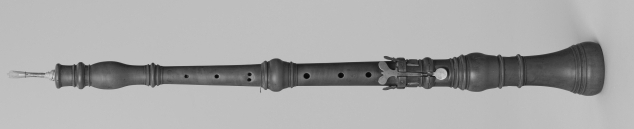
\includegraphics[width=0.9\textwidth]{06someJpgOboeBaroqueDennerMIR370.jpg}%
\end{center}
\caption{\label{fig:asIsJpg}Some jpg-picture, directly included }
\end{figure}

\begin{figure}[htb]
\begin{center}
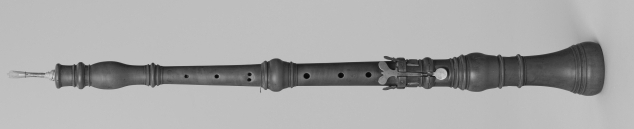
\includegraphics[width=0.9\textwidth]{07somePngOboeBaroqueDennerMIR370.png}%
\end{center}
\caption{\label{fig:asIsPng}Some png-picture, directly included }
\end{figure}


Figure \ref{fig:asIsSvg} is a picture in \gls{svg}-format 
and included directly. 
This time, we did not use the {\tt graphicx}-package 
but the package {\tt svg}. 
Inclusion is with the {\tt\textbackslash includesvg}-command. 
Note that the suffix of the filename shall be omitted. 
So the command is {\tt \textbackslash
includesvg[width=0.9\textbackslash textwidth]\{some\}}. 
For more information see \cite{SvgP}. 
Caution: {\tt inkscape} must be installed. 

\begin{figure}[htb]
\begin{center}
\includesvg[width=0.9\textwidth]{08someSvg}%
\end{center}
\caption{\label{fig:asIsSvg}Some svg-picture, directly included }
\end{figure}

\subsection{Transforming (la)tex-files into pdf-files}\label{subsec:tex2pdf}

The next step is to create a pdf-file from the tex-files. 
LaTeX distinguishes master tex-files from tex-files intended to be inputted
from elsewhere. 
Master tex-files have the form 
%
\lstset{language=tex, basicstyle=\small}
\begin{lstlisting}
\documentclass{...}

\begin{document}
...
\end{document}
\end{lstlisting}

To satisfy this task, one may apply a latex to pdf converter {\tt latex2pdf} 
to a master tex-file {\tt xxx.tex}. 
The latex to pdf converter {\tt latex2pdf} 
is configurable via the parameter {\tt texCommand} 
(misleading name, I know, but short). 
Possible values are {\tt pdflatex}, {\tt lualatex} and {\tt xelatex}, 
where the first is the default for which this software is also tested. 
It is also possible to pass parameters to the latex to pdf converter. 

In fact, the converter {\tt latex2pdf} 
does much more than converting tex to pdf. 
Figure \ref{fig:tex2pdf} shows for {\tt latex2pdf} set to {\tt pdflatex}, 
that besides the pdf-file also a log-file and an aux-file is created. 
The log-file contains logging information on the run of the conversion 
and the aux-file transports information from one run to the next. 
Thus conversion goes without it but it is read if present. 
This is why it is depicted at input side in dashed lines. 

What is in fact in the aux-file depends on the package. 
Among other information, 
also citations and the location of the bibliography file with ending bib 
are present. 
This cannot be used directly in the next {\tt latex2pdf} run 
to create the bibiography, 
because the entries must be retrieved from the bib-file, 
collected and sorted. 
This is done by invoking {\tt bibtex} between two {\tt latex2pdf} runs. 
Based on the aux-file, {\tt bibtex} creates a bbl-file 
containing the bibliography, which is read in in the next {\tt latex2pdf} run. 
For details see Section \ref{subsec:bibtex}. 

If an index is demanded, in addition {\tt latex2pdf} creates an \gls{idx}-file. 
As the citations, it cannot be used directly to create an index in
the next {\tt latex2pdf} run, 
because the index entries must be collected and sorted before. 
This is done by invoking {\tt makeindex} between the two {\tt latex2pdf} runs. 
Based on the idx-file, {\tt makeindex} creates an \gls{ind}-file 
containing the index, which is read in in the next {\tt latex2pdf} run. 
For details see Section \ref{subsec:indices}. 

If a glossary is demanded, this can be read off the \gls{aux}-file 
and a \gls{glo}-file is created. 
As the index, it cannot be used directly to create a glossary in
the next {\tt latex2pdf} run, 
because the glossary entries must be collected and sorted before. 
This is done by invoking {\tt makeglossaries} 
between the two {\tt latex2pdf} runs. 
Based on the glo-file, {\tt makeglossaries} creates a \gls{gls}-file 
containing the glossary, which is read in in the next {\tt latex2pdf} run. 
For details see Section \ref{subsec:glossaries}. 

In addition, 
if a table of contents, a list of figures or a list of tables is required, 
also a toc-file, a lof-file and a lot-file is created 
collecting the according information. 
If such a file is present, it is read in 
and is used to create a table of contents, a list of figures and of tables 
in the second run of {\tt latex2pdf}. 

To summarize, 
if a table of contents, a list of figures, a list of tables or 
a bibliography, an index or a glossary is present, 
a second latex run is required to make them appear in the pdf-output. 

If a table of contents and at the same time 
a bibliography, an index or a glossary is present, 
even two further latex runs are required: 
After the first one, the bibliography, the index or the glossary 
occurs in the pdf-file but not yet in the table of contents. 
This happens after the second additional latex run. 

\begin{figure}[htb]
\begin{center}
\input{09tex2pdf.ptx}
\end{center}
\caption{\label{fig:tex2pdf}Conversion of a tex-file into a pdf-file}
\end{figure}

\subsection{Bibliographies}\label{subsec:bibtex}

In case the latex to pdf converter writes bibliographic information, 
into its aux-file, a bibliography must be generated. 
Bibliographic information are 
citations, a link to the bib-file containing the bibliography data, 
and optionally a link to the bibliography style file. 

To create a bibliography, a {\tt bibtex}-command must be run. 
Essentially, {\tt bibtex} extracts the citations in the aux-file, 
unifies them, 
retrieves the according entries from the bib-file, sorts these 
and writes them into a bbl-file 
which can be included in the next run of {\tt latex2pdf}. 

This software presupposes, that {\tt bibtex} reads the aux-file 
and creates a bbl-file and also an blg-file with logging output 
as illustrated by Figure \ref{fig:aux2bbl}. 
From the blg-file this software may determine 
whether {\tt bibtex} emitted an error or warnings. 


\begin{figure}[htb]
\begin{center}
\input{10aux2bbl.ptx}
\end{center}
\caption{\label{fig:aux2bbl}
Conversion of an aux-file into a bbl-file using a bibliography}
\end{figure}

Vital information on {\tt bibtex} can be found in \cite{BibPat} 
and in \cite{BibMar}. 
Also Chapter 10 in \cite{Gra} gives vital information on {\tt bibtex}. 


\subsection{Indices}\label{subsec:indices}

Note that despite of the headline of this section, 
only a single index is supported and this requires 
the package {\tt makeidx} described in \cite{MkidxShIdxP}. 
For an extension see Section \ref{sec:gaps}. 

Interesting enough, 
the commands {\tt\textbackslash index} and {\tt\textbackslash makeindex} 
work even without using the package {\tt makeidx}. 
The former essentially does nothing without the latter
but if the latter is present, if {\tt xxx.tex} is the latex main file, 
the former writes an according entry in a file {\tt xxx.idx}. 
Essentially, 
{\tt\textbackslash makeindex} prepares writing to the \gls{idx}-file, 
whereas {\tt\textbackslash index} performs writing a line. 
For example {\tt\textbackslash index\{ant-task\}} creates an entry 
%
\begin{verbatim}
\textbackslash indexentry\{ant-task|hyperpage\}\{3\}
\end{verbatim}
%
in {\tt xxx.idx}. 
Note that {\tt xxx.idx} typically contains entries more than once 
and that the entries are not sorted. 
 
Running, the {\tt makeindex}-command performs sorting 
and typically also unification. 
Essentially, {\tt makeindex} sorts and combines index entries. 
This software presupposes, that {\tt makeindex} converts the idx-file 
into an ind-file containing the index 
and creating also an ilg-file with logging output 
as shown in Figure \ref{fig:idx2ind}. 
From the ilg-file this software may determine 
whether {\tt makeindex} emitted an error or warnings. 

The package {\tt makeidx} provides a single command, 
{\tt\textbackslash printindex} which reads in the ind-file 
and prints the index in a separate section, 
typically at the end of the pdf-file. 
The package {\tt tocbibind} described in \cite{TocBibIndP}, 
then writes the headline of the index into the table of contents. 
\index{table of contents}

In case the latex to pdf converter creates an idx-file, 
an index must be generated. 
% Well, this is not really the truth: it is needed only if ...

\begin{figure}[htb]
\begin{center}
\input{11idx2ind.ptx}
\end{center}
\caption{\label{fig:idx2ind}Conversion of an idx-file into an ind-file}
\end{figure}

It is possible to configure the makeindex-command 
and to pass arbitrary options. 
CAUTION: For the usual {\tt makeindex}-command, 
the options {\tt -o} specifying an output file 
and {\tt -t} (transcript) specifying the logging file are not allowed, 
because this breaks the expectation to find the sorted index 
in file {\tt xxx.ind} 
and bypasses the detection of errors and warnings of this software, 
respectively. 
Also specifying a style file via option {\tt -s} 
is not recommended because this is used to create a glossary 
and so breaks glossary creation 
as described in Section \ref{subsec:glossaries}. 

Information on the makeindex program can be found in \cite{MkIdxMoe} 
and in \cite{MkIdxLam}. 
Also there is a site \cite{MakeIdxOpts} 
describing all available options for {\tt makeindex}. 



\subsection{Glossaries}\label{subsec:glossaries}

Creating glossaries 
requires the package {\tt glossaries} described in \cite{GloP}. 
Note that despite of the headline of this section, 
an despite {\tt glossaries} itself supports multiple glossaries, 
this software supports only a single glossary 
and also sorting and unifying is done 
either via {\tt makeindex} as for indices or via {\tt xindy}, 
whereas the option to do without external programs 
offered also by package {\tt glossaries} 
is not supported by this software. 

For generalizations see Section \ref{sec:gaps}. 

As for creating indices there is a latex-command {\tt\textbackslash makeindex}, 
to create a glossary there is a latex-command 
{\tt\textbackslash makeglossaries} 
but the latter is not builtin as {\tt\textbackslash makeindex} 
but provided by the package {\tt glossaries}. 
If {\tt xxx.tex} is the latex main file, 
{\tt\textbackslash makeglossaries} opens the glo-file {\tt xxx.glo} 
containing glossary entries for writing. 
As the builtin command {\tt\textbackslash index} 
writes entries into the idx-file defining the index, 
the command {\tt\textbackslash gls} defined by the package {\tt glossaries} 
writes an entry into the glo-file. 
Note that {\tt xxx.glo} typically contains entries more than once 
and that the entries are not sorted. 



To perform sorting and typically also unification, 
the package {\tt glossaries} allows three mechanisms. 
This software supports two of them: 
via the shell command {\tt makeindex} as used for indices
and via the shell command {\tt xindy}. 
Using {\tt makeindex} is the default but can also be activated through 
{\tt\textbackslash usepackage[makeindex]\{glossaries\}}. 
Using {\tt xindy} is triggered through 
{\tt\textbackslash usepackage[xindy]\{glossaries\}}. 
Accordingly, for {\tt makeindex} the aux-file receives lines 
%
\begin{verbatim}
\providecommand\@istfilename[1]{}
\@istfilename{manualLatexMavenPlugin.ist}
\end{verbatim}
%
whereas for {\tt xindy}, there are lines 
%
\begin{verbatim}
\providecommand\@istfilename[1]{}
\@istfilename{manualLatexMavenPlugin.xdy}
...
\providecommand\@xdylanguage[2]{}
\@xdylanguage{main}{english}
\providecommand\@gls@codepage[2]{}
\@gls@codepage{main}{}
\end{verbatim}



This software neither invokes {\tt makeindex} nor {\tt xindy} directly. 
Instead it invokes the shell command {\tt\textbackslash makeglossaries}
(which is invoked without file ending)  
which determines from the aux-file 
whether to invoke {\tt makeindex} nor {\tt xindy}. 
Accordingly, it writes the style definition 
by creating an ist-file {\tt xxx.ist} or an xdy-file {\tt xxx.xdy} 
if {\tt makeindex} or {\tt xindy} is specified as package option, 
respectively. 

Seemingly, {\tt\textbackslash makeglossaries} relies on the aux-file 
to determine whether to invoke {\tt makeindex} or {\tt xindy} 
for sorting and unification. 
Then it invokes the according command and writes a log-file 
with ending {\tt glg}, 
redirecting the logging output of {\tt makeindex} or {\tt xindy} 
adding own output so that a glg-file may be written, 
even if e.g. {\tt makeindex} is invoked and does not. 
In any case, if the glg-file is written, 
{\tt\textbackslash makeglossaries} writes text matching 
%
\begin{verbatim}
(^\*\*\* unable to execute: )
\end{verbatim}
%
in the glg-file if an error occurs, 
no matter whether {\tt makeindex} or {\tt xindy} is invoked. 
Possibly, there are cases where an error causes no glg-file to be written. 
If no error occurs, a glg-file is written 
and if warnings are emitted, 
they either come from {\tt makeindex} or from {\tt xindy}. 
Thus warnings may be detected with the patterns 
defined by {\tt makeindex} and by {\tt xindy}. 

The style {\tt list} (which is the default) is set in the form 
%
\begin{verbatim}
\usepackage[style=list]{glossaries}
\end{verbatim}
%
where \cite{GloP}, Section 15 lists predefined styles. 
So, the style determines the content of the style definition, 
whereas the options {\tt makeindex} and {\tt xindy} 
specify the form in which the style is encoded 
and thus the ending of the style file, which is either {\tt ist} or {\tt xdy}. 

Sorting the glo-file, as said above, 
currently is only supported using {\tt makeglossaries}. 
The allowed options are essentially those 
making sense for {\tt makeindex} and those making sense for {\tt xindy}. 
If the shell command {\tt makeglossaries} 
invokes {\tt makeindex} of course only the according options 
are passed supplemented by additional options 
{\tt -s}, {\tt -t}, {\tt -o}, to specify the
ist-file, the log-file (the transcript-file) and the gls-file 
which is the result of sorting, the output file, 
and contains the entries of the glo-file 
just sorted, formatted and unified. 
Accordingly, if the shell command {\tt makeglossaries} 
invokes {\tt xindy} of course only the according options 
are passed supplemented by additional options 
{\tt -M}, {\tt -t}, {\tt -o}. 
This is illustrated in Figure \ref{fig:glo2gls}. 


\begin{figure}[htb]
\begin{center}
\input{12glo2gls.ptx}
\end{center}
\caption{\label{fig:glo2gls}Conversion of a glo-file into a gls-file 
using {\tt makeglossaries}}
\end{figure}



\subsection{Rerunning the latex processor}\label{subsec:rerunLatex}

As indicated in the previous sections, 
{\tt latex2pdf} must be rerun, if {\tt bibtex} or {\tt makeindex} had been run 
to read in the bibliography created by {\tt bibtex} 
or the index created by {\tt makeindex}. 
Likewise, if a toc-file, a lof-file or a lot-file 
had been created in the first {\tt latex2pdf} run, 
another run is needed to read in these files 
to create a table of contents, a list of figures or a list of tables, 
respectively. 
Note that for all these cases, 
the log-file does not allow to detect that {\tt latex2pdf} has to be rerun, 
by matching a fixed pattern. 

After the second run of {\tt latex2pdf}, 
the table of contents is included and the references and citations are
inserted 
which may shift the subsequent text 
which may require another run of {\tt latex2pdf} 
This may be detected by pattern matching on the log-file. 

Note that there are several packages which require additional runs, 
such as the longtable-package, 
which may vary dimensions of tables. 
This software presupposes, that all these reruns 
may be detected by matching a fixed pattern in the log-file. 
Since packages are frequently changed and new packages are written, 
also the pattern cannot be fixed. 
Thus it is configurable. 

Note that, if a package requires running other programs 
between two runs of {\tt latex2pdf}, 
this would require a change in this software. 


\subsection{Creating hypertext}\label{subsec:tex2html}

To create html and xhtml from latex files, 
a {\tt htlatex}-command is used. 
This may be {\tt htlatex}, the default based on {\tt latex} 
and {\tt htxelatex} based on {\tt xelatex}. 

Figure \ref{fig:tex2xml} shows the steps {\tt htlatex} performs: 
From the input latex file {\tt xxx.tex} 
another latex file {\tt yyy.tex} is created 
which arises from {\tt xxx.tex} by adding 
{\tt \textbackslash usepackage[...]\{tex4ht\}}. 
Then {\tt htlatex} runs {\tt latex} on {\tt yyy.tex} 
which results in {\tt yyy.dvi}. 
Note that this is in contrast to {\tt pdflatex} 
which would create some {\tt yyy.pdf}. 

Then comes the converter {\tt tex4ht} into the game 
which creates several html-files among those also {\tt xxx.html}. 
The other files, {\tt yyy.idv} and {\tt yyy.lg}, 
are further processed by {\tt t4ht} 
creating the stylesheet {\tt xxx.css} and graphic files. 

The output of TeX is a standard \gls{dvi}-file 
interleaved with special instructions for the postprocessor tex4ht to use. 
The special instructions come from implicit and explicit requests 
made in the source file through commands of TeX4ht.

The utility {\tt tex4ht} translates the dvi-code into standard text, 
while obeying the requests it gets from the special instructions. 
The special instructions may request the creation of files, 
insertion of html code, filtering of pictures, and so forth. 
In the extreme case that the source code contains no commands of TeX4ht, 
{\tt tex4ht} gets pure dvi-code and it outputs (almost) plain text 
with no hypertext elements in it.

The special ({\tt\textbackslash special}) instructions seeded in the dvi-code 
are not understood by dvi processors other than those of TeX4ht.


{\tt xxx.idv}
This is a dvi-file extracted from {\tt xxx.dvi}, 
and it contains the pictures needed in the html files.

{\tt xxx.lg}
This is a log file listing the pictures of {\tt xxx.idv}, 
the \gls{png} files that should be created, CSS information, 
and user directives introduced 
through the ‘{\tt\textbackslash Needs\{...\}}’ command.


{\tt t4ht}
This is an interpreter 
for executing the requests made in the {\tt xxx.lg} script.

\begin{figure}[htb]
\begin{center}
\input{13tex2xml.ptx}
\end{center}
\caption{\label{fig:tex2xml}Conversion of a tex-file into an xml-file}
\end{figure}

\subsection{Creating odt-files}\label{subsec:tex2odt}

\subsection{Creating MX word files}\label{subsec:tex2doc}

The best way to convert latex files into MS word files is via odt files. 
Conversion from latex to odt 
is already described in Section \ref{subsec:tex2odt}. 
The last step can be done by {\tt odt2doc} which can create both 
doc-format and docx-format and many others 
which is illustrated in Figure \ref{fig:tex2doc}. 


\begin{figure}[htb]
\begin{center}
\input{14tex2doc.ptx}
\end{center}
\caption{\label{fig:tex2doc}Conversion of a tex-file into a docx-file}
\end{figure}



\subsection{Creating plain text files}\label{subsec:tex2txt}

Why should one create plain text from latex files? 
Maybe this is the minimal format the receiver can work with. 
Another common application is wordcount, 
in particular if writing a paper for a journal. 

Plain text files can be created from latex files 
just by stripping off the tex-commands. 
The disadvantage is, 
that references, bibliography, index, glossary, 
table of contents, list of figures, list of tables, \dots 
and symbols get lost. 
Thus, the first step we take is complete creation of a pdf-file 
except display of warnings like bad boxes 
as described in Section \ref{subsec:tex2pdf}. 
This creates an appropriate pdf-file, 
with correct numberings and links, 
possibly with overfull boxes and that like. 
As a final step, we convert the pdf-file into a text file 
using, as a default {\tt pdftotext} with ending {\tt txt}. 
Figure \ref{fig:tex2txt} illustrates the translation process. 

\begin{figure}[htb]
\begin{center}
\input{15tex2txt.ptx}
\end{center}
\caption{\label{fig:tex2txt}Conversion of a tex-file into an txt-file}
\end{figure}

Note that {\tt pdftotext} produces a text file with page numbers 
and signifies the end of a page 
(to see how, just have a look at the end of the file), 
so that one can identify page numbers as such. 
Thus references, index, glossary, table of contents and that like 
referring to page numbers carry valuable information. 
Also symbols available in utf8 encoding are preserved. 
In contrast, heavily stacked formulae become unreadable, 
because {\tt pdftotext} displays them line by line 
and drops fraction bars completely. 
Also formulae with complex subformulae in a root operator  
become unreadable because the root operator becomes just a root symbol. 
Likewise for integrals and that like. 

Aspects of figures kept are the captions of course but also the latex-texts. 
This is displayed linewise. 
What gets lost is the postscript/pdf-parts, i.e. the plain graphics. 



\subsection{Miscellaneous}

Warning of failures occurs each time pdflatex is run. 
Restricting this to the first run is not appropriate, 
because the aux-file is read and so the failures may depend on the run. 






%\index{!!!!}
%\index{bla|(}
%\index{bla|)}





How to work on: First step: %
\begin{verbatim}
<cleanUp>false</cleanUp>
\end{verbatim}
Then have a look at the logging file. 


\section{Settings}\label{sec:settings}

This section describes the parameters 
of both the ant-task and the maven-plugin. 
After an overview in Section \ref{subsec:settingsOverview}, 
We give in depth explanations in Section \ref{subsec:settingsDetail}. 

\section{Overview and Listings}\label{subsec:settingsOverview}

First we provide a table, Table \ref{tab:parameters} 
with parameter names, default values 
and explanation, then listings of the configuration 
in the {\tt pom.xml} for the maven-plugin 
and in the {\tt build.xml} for the ant-task. 
The listing of the {\tt build.xml} shows 
which parameters are attributes and which ones are text elements. 
In {\tt pom.xml} only text elements occur. 
Note that neither of the parameters is mandatory, 
as there are always valid default values. 


\begin{longtable}{|ll|}
\hline
Parameter        & Default  \\
\multicolumn2{|l|}{Explanation }  \\
\hline
\hline
\multicolumn2{|l|}{directories, miscellaneous } \\
\hline
\tt texSrcDirectory  & \tt src/site/tex  \\
\multicolumn2{|l|}{
\begin{minipage}{0.95\linewidth}
The tex source directory as a string, 
containing all tex main documents 
(including subfolders) to be processed
relative to {\tt\$baseDirectory}. 
The default value is '{\tt src/site/tex}' on Unix systems. 
\end{minipage}
} \\
\tt outputDirectory  & \tt .             \\
\multicolumn2{|l|}{
\begin{minipage}{0.95\linewidth}
The generated artifacts will be copied to {\tt outputDirectory}
relative to {\tt\$targetSiteDirectory} 
which is by default '{\tt\$targetDirectory/site}' on Unix systems. 
%The default value is '{\tt.}'.  
\end{minipage}
} \\
\tt targets          & \tt pdf, html     \\
\multicolumn2{|l|}{
\begin{minipage}{0.95\linewidth}
A comma separated list of targets to be stored in {\tt\$targetSet}. 
%The default value is '{\tt pdf, html}'. 
\end{minipage}
} \\
\tt targets          & \tt pdf, html     \\
\multicolumn2{|l|}{
\begin{minipage}{0.95\linewidth}
A comma separated list of targets to be stored in {\tt\$targetSet}. 
%The default value is '{\tt pdf, html}'. 
\end{minipage}
} \\
\tt patternLatexMainFile          &  \textbackslash s*\textbackslash (documentstyle|documentclass).*        \\
\multicolumn2{|l|}{
\begin{minipage}{0.95\linewidth}
The pattern which identifies a latex main file. 
If the default value is not appropriate, please modify 
and notify the developer of this plugin. 
\end{minipage}
} \\
\tt fig2devCommand   & \tt fig2dev  \index{fig2dev}     \\
\multicolumn2{|l|}{
\begin{minipage}{0.95\linewidth}
The fig2dev command for conversion of fig-files into various formats. 
Currently only {\tt pdf} combined with {\tt ptx} is supported. 
%The default value is '{\tt fig2dev}'. 
\end{minipage}
} \\
\hline
\multicolumn2{|l|}{latex to pdf} \\
\hline
\tt texCommand       & \tt pdflatex      \\
\multicolumn2{|l|}{
\begin{minipage}{0.95\linewidth}
The LaTeX command to create a pdf-file with. 
%The default value is '{\tt pdflatex}'. 
\end{minipage}
} \\
\tt texCommandArgs   & see below  \\%\tt\small -interaction=nonstopmode -src-specials
\multicolumn2{|l|}{
\begin{minipage}{0.95\linewidth}
The arguments string to use 
when calling LaTeX via {\tt\$texCommand}.
Leading and trailing blanks are ignored. 
A sequence of at least one blank separate the proper options. 
%The default value is 
%'{\tt-interaction=nonstopmode -src-specials}'. 
\end{minipage}
} \\
\tt patternErrLatex & \tt(\^{}! ) \\
\multicolumn2{|l|}{
\begin{minipage}{0.95\linewidth}
The pattern in the log-file 
indicating a failure when running the {\tt\$texCommand}. 
%The default value is 
%'{\tt ! $|$Fatal error$|$LaTeX Error$|$Emergency stop}'. 
If this is not complete, please extend 
and notify the developer of this plugin. 
\end{minipage}
} \\
\tt debugbadboxes    & \tt true          \\
\multicolumn2{|l|}{
\begin{minipage}{0.95\linewidth}
Whether debugging of overfull/underfull hboxes/vboxes is on: 
If so, a bad box occurs in the last LaTeX run, a warning is displayed. 
For details, set {\tt\$cleanUp} to false, 
rerun LaTeX and have a look at the log-file.
%The default value is '{\tt true}'. 
\end{minipage}
} \\
\tt debugwarnings    & \tt true          \\
\multicolumn2{|l|}{
\begin{minipage}{0.95\linewidth}
Whether debugging of warnings is on: 
If so, a warning in the last LaTeX run is displayed. 
For details, set {\tt\$cleanUp} to false, 
rerun LaTeX and have a look at the log-file. 
%The default value is '{\tt true}'. 
\end{minipage}
} \\
\hline
\multicolumn2{|l|}{bibtex} \\
\hline
\tt bibtexcommand    & \tt bibtex        \\
\multicolumn2{|l|}{
\begin{minipage}{0.95\linewidth}
The BibTeX command to create a bbl-file 
from an aux-file and a bib-file (using a bst-style file). 
%The default value is '{\tt bibtex}'. 
\end{minipage}
} \\
\tt patternErrBibtex    & \tt error message        \\
\multicolumn2{|l|}{
\begin{minipage}{0.95\linewidth}
The Pattern in the blg-file 
indicating that \$bibtexCommand failed. 
The default value is chosen 
according to the 'bibtex' documentation. 
\end{minipage}
} \\
\tt patternWarnBibtex    & \tt Warning-{}-        \\
\multicolumn2{|l|}{
\begin{minipage}{0.95\linewidth}
The Pattern in the blg-file 
indicating a warning \$bibtexCommand emitted. 
The default value is chosen 
according to the 'bibtex' documentation. 
\end{minipage}
} \\
\hline
\multicolumn2{|l|}{makeindex} \\
\hline
\tt makeIndexCommand & \tt makeindex     \\
\multicolumn2{|l|}{
\begin{minipage}{0.95\linewidth}
The MakeIndex command to create an ind-file from an idx-file 
logging on an ilg-file. 
%The default value is '{\tt makeindex}'. 
\end{minipage}
} \\
\tt makeIndexOptions & the empty string     \\
\multicolumn2{|l|}{
\begin{minipage}{0.95\linewidth}
The options for the MakeIndex command. 
% The default value is the empty string. 
\end{minipage}
} \\
\tt patternErrMakeindex & \tt (!! Input index error )        \\
\multicolumn2{|l|}{
\begin{minipage}{0.95\linewidth}
The pattern in the ilg-file 
indicating that \$makeIndexCommand failed. 
The default value is chosen 
according to the 'makeindex' documentation.
\end{minipage}
} \\
\tt patternWarnMakeindex & \tt (\#\# Warning )        \\
\multicolumn2{|l|}{
\begin{minipage}{0.95\linewidth}
The pattern in the ilg-file 
indicating a warning \$makeIndexCommand emitted. 
The default value is chosen 
according to the 'makeindex' documentation.
\end{minipage}
} \\
\hline
\multicolumn2{|l|}{makeglossaries} \\
\hline
\tt makeGlossariesCommand & \tt makeglossaries         \\
\multicolumn2{|l|}{
\begin{minipage}{0.95\linewidth}
The MakeGlossaries command to create a gls-file 
from a glo-file (invoked without file ending) 
also taking ist-file or xdy-file 
into account logging on a glg-file. 
\end{minipage}
} \\
\tt makeGlossariesOptions & the empty string          \\
\multicolumn2{|l|}{
\begin{minipage}{0.95\linewidth}
The options for the \$makeGlossariesCommand. 
These are the options for 'makeindex' (not for \$makeIndexCommand) 
and for 'xindy' (also hardcoded). 
The aux-file decides on whether program is executed 
and consequently which options are used. 
		 
The default value is the empty option string. 
Nevertheless, 'xindy' is invoked as 'xindy -L english  -I xindy -M ...'. 
With option '-L german', this is added. 
Options '-M<' for 'xindy' 
'-s' for 'makeindex</code> and '-t' and '-o' for both, 'xindy' and 'makeindex'. 
\end{minipage}
} \\
\tt patternMakeGlossariesErr & 
\tt(\^\textbackslash*\textbackslash*\textbackslash* unable to execute: ) \\
\multicolumn2{|l|}{
\begin{minipage}{0.95\linewidth}
The Pattern in the glg-file 
indicating an error when running \$makeGlossariesCommand. 
If the default value is not appropriate, please modify 
and notify the developer of this plugin. 
\end{minipage}
} \\
\tt patternErrXindy & \tt (\^ERROR: )         \\
\multicolumn2{|l|}{
\begin{minipage}{0.95\linewidth}
The pattern in the 'glg' file 
indicating an error when running 'xindy' 
via \$makeGlossariesCommand. 
If the default value is not appropriate, please modify 
and notify the developer of this plugin. 
\end{minipage}
} \\
\tt patternWarnXindy & \tt (\^WARNING: )         \\
\multicolumn2{|l|}{
\begin{minipage}{0.95\linewidth}
The pattern in the 'glg' file 
indicating a warning when running 'xindy' 
via \$makeGlossariesCommand. 
If the default value is not appropriate, please modify 
and notify the developer of this plugin. 
\end{minipage}
} \\
\hline
\multicolumn2{|l|}{htlatex} \\
\hline
\tt tex4htCommand       & \tt htlatex  \\
\multicolumn2{|l|}{
\begin{minipage}{0.95\linewidth}
\end{minipage}
} \\
\tt tex4htStyOptions    & \tt xhtml,uni-html4,2,svg  \\
\multicolumn2{|l|}{
\begin{minipage}{0.95\linewidth}
\end{minipage}
} \\
\tt tex4htOptions       & \tt -cunihtf -utf8         \\
\multicolumn2{|l|}{
\begin{minipage}{0.95\linewidth}
\end{minipage}
} \\
\tt t4htOptions         & the empty string              \\%-cvalidate
\multicolumn2{|l|}{
\begin{minipage}{0.95\linewidth}
The options for 't4ht' which converts idv-file and lg-file 
into css-files, tmp-file and, 
by need and if configured accordingly into \gls{png}-files. 
The value '-p' prevents creation of \gls{png}-pictures.
%The default value is the empty string. 
\end{minipage}
} \\
\tt patternLatexNeedsReRun &  see below ****          \\
\multicolumn2{|l|}{
\begin{minipage}{0.95\linewidth}
The pattern in the log file which triggers rerunning latex. 
This pattern may never be ensured to be complete, 
because any new package may break completeness. 
Nevertheless, the default value aims completeness 
while be restrictive enough not to trigger another latex run if not needed. 
To ensure termination, let \$maxNumReruns 
specify the maximum number of latex runs. 
If the user finds an extension, (s)he is asked to contribute 
and to notify the developer of this plugin. 
Then the default value will be extended. 
\end{minipage}
} \\
\tt maxNumReruns        & \tt 5               \\
\multicolumn2{|l|}{
\begin{minipage}{0.95\linewidth}
The maximal allowed number of reruns of the latex process. 
This is to avoid endless repetitions. 
%The default value is 5. 
This shall be non-negative 
or -1 which signifies that there is no threshold. 
\end{minipage}
} \\
\tt latex2rtfCommand    & \tt latex2rtf        \\
\multicolumn2{|l|}{
\begin{minipage}{0.95\linewidth}
The latex2rtf command to create rtf from latex directly. 
%The default value is '{\tt latex2rtf}'. 
\end{minipage}
} \\
\tt odt2docCommand      & \tt odt2doc          \\
\multicolumn2{|l|}{
\begin{minipage}{0.95\linewidth}
The odt2doc command to create MS word-formats from otd-files. 
%The default value is '{\tt odt2doc}'. 
\end{minipage}
} \\
\tt odt2docOptions      & \tt -fdocx          \\
\multicolumn2{|l|}{
\begin{minipage}{0.95\linewidth}
The options of the odt2doc command. 
Above all specification of output format via the option '-f'. 
The odt2doc command is invoked in the form 
'{\tt odt2doc -f$<$format$>$ $<$file$>$.odt}'. 
All output formats are shown by '{\tt odt2doc --show}' 
but the formats interesting in this context 
are the following: 
{\tt doc}, {\tt doc6}, {\tt doc95}, {\tt docbook}, {\tt docx}, 
{\tt docx7}, {\tt ooxml} and {\tt rtf}. 
Interesting also the verbosity options '{\tt -v}', '{\tt -vv}', '{\tt -vvv}' 
the timeout '{\tt -T=secs}' and '{\tt --preserve}' 
to keep permissions and timestamp of the original document. 
%The default value is '{\tt -fdocx}'. 
\end{minipage}
} \\
\tt pdf2txtCommand      & \tt pdftotext        \\
\multicolumn2{|l|}{
\begin{minipage}{0.95\linewidth}
The pdf2txt command converting pdf into plain text. 
%The default value is '{\tt pdftotext}'. 
\end{minipage}
} \\
\tt pdf2txtOptions      & the empty string  \\
\multicolumn2{|l|}{
\begin{minipage}{0.95\linewidth}
The options of the pdf2txt command. 
%The default value is the empty string. 
\end{minipage}
} \\
\tt cleanUp             & \tt true             \\
\multicolumn2{|l|}{
\begin{minipage}{0.95\linewidth}
Clean up the working directory in the end? 
May be used for debugging when setting {\tt false}. 
%The default value is '{\tt true}'. 
\end{minipage}
} \\
\hline
\caption{\label{tab:parameters} The parameters of task and plugin }
\end{longtable}



The maven-plugin described here, 
requires the following definition in {\tt pom.xml}. 

\lstset{language=xml, basicstyle=\scriptsize}
\begin{lstlisting}
<!-- create html and pdf and other formats from latex -->
<plugin>
  <groupId>de.akquinet.jbosscc.latex</groupId>
  <artifactId>latex-maven-plugin</artifactId>
  <version>1.3-SNAPSHOT</version><!--uptodate?-->
  <!--artifactId>maven-latex-plugin</artifactId>
      <version>1.2</version--><!--uptodate?-->
  <configuration>
  <settings>
  <!-- The tex source directory as a string, containing 
       all tex main documents (including subfolders) to be processed 
       relative to $baseDirectory. 
       The default value is 'src/site/tex' on Unix systems. -->
    <texSrcDirectory>src/site/tex</texSrcDirectory>

    <!-- The generated artifacts will be copied to this folder 
	 relative to $targetSiteDirectory 
	 which is by default '$targetDirectory/site' on Unix systems. 
	 The default value is '.'.  -->
    <outputDirectory>.</outputDirectory>

    <!-- A comma separated list of targets 
	 to be stored in $targetSet. 
	 The default value is 'pdf, html'. -->
    <targets>pdf, html</targets>

    <!-- The pattern which identifies a latex main file. 
	 The default value is '\s*\\(documentstyle|documentclass).*'. 
	 If this is not appropriate, please modify 
	 and notify the developer of this plugin. -->
    <patternLatexMainFile>
      \s*\\(documentstyle|documentclass).*
    </patternLatexMainFile>

    <!-- Path to the TeX scripts or null. 
	 In the latter case, the scripts must be on the system path. 
	 Note that in the pom, <texPath/> 
	 and even <texPath>    </texPath> represent the null-File. 
	T he default value is null. -->
    <texPath/> 

    <!-- The fig2dev command for conversion of fig-files 
	 into various formats. 
	 Currently only pdf combined with ptx is supported. 
	 The default value is 'fig2dev'.  -->
    <fig2devCommand>fig2dev</fig2devCommand>
  
    <!-- The LaTeX command to create a pdf-file. 
	 The default value is 'pdflatex'. -->
    <texCommand>pdflatex</texCommand>

    <!-- The arguments string to use 
         when calling latex via $texCommand 
         Leading and trailing blanks are ignored. 
	 A sequence of at least one blank separate the proper options. 
	 The default value is 
	 '-interaction=nonstopmode -synctex=1 -src-specials 
	  -recorder -shell-escape'. -->
    <texCommandArgs>
      -interaction=nonstopmode 
      -synctex=1 
      -src-specials 
      -recorder 
      -shell-escape 
    </texCommandArgs>

    <!-- The pattern in the log-file 
	 indicating a failure when running $texCommand. 
	 The default value is 
	 '(^! )'. 
	 If this is not complete, please extend 
	 and notify the developer of this plugin. -->
    <patternErrLatex>(\^! )</patternErrLatex>

    <!-- Whether debugging of overfull/underfull hboxes/vboxes is on: 
	 If so, a bad box occurs in the last LaTeX run, 
	 a warning is displayed. 
	 For details, set $cleanUp to false, 
	 rerun LaTeX and have a look at the log-file.
	 The default value is 'true'. -->
    <debugBadBoxes>true</debugBadBoxes>

    <!-- Whether debugging of warnings is on: 
	 If so, a warning in the last LaTeX run is displayed. 
	 For details, set $cleanUp to false, 
	 rerun LaTeX and have a look at the log-file. 
	 The default value is 'true'. -->
    <debugWarnings>true</debugWarnings>

    <!-- The BibTeX command to create a bbl-file 
	 from an aux-file and a bib-file (using a bst-style file). 
	 The default value is 'bibtex'. -->
    <bibtexCommand>bibtex</bibtexCommand>

    <!-- The Pattern in the blg-file 
	 indicating that $bibtexCommand failed. 
	 The default value is chosen 
	 according to the 'bibtex' documentation. -->
    <patternErrBibtex>error message</patternErrBibtex>

    <!-- The Pattern in the blg-file 
	 indicating a warning $bibtexCommand emitted. 
	 The default value is chosen 
	 according to the 'bibtex' documentation. -->
    <patternWarnBibtex>Warning--</patternWarnBibtex>

    <!-- The MakeIndex command to create an ind-file 
	 from an idx-file logging on an ilg-file. 
	 The default value is 'makeindex'. -->
    <makeIndexCommand>makeindex</makeIndexCommand>

    <!-- The options for the MakeIndex command. 
	 The default value is the empty string. -->
    <makeIndexOptions></makeIndexOptions>

    <!-- The pattern in the ilg-file 
	 indicating that $makeIndexCommand failed. 
	 The default value '(!! Input index error )' 
	 is chosen according to the 'makeindex' documentation.  -->
    <patternErrMakeindex>(!! Input index error )</patternErrMakeindex>
 
    <!-- The Pattern in the ilg-file 
	 indicating a warning $makeIndexCommand emitted. 
	 The default value '(## Warning )' 
	 is chosen according to the 'makeindex' documentation. -->
    <patternWarnMakeindex>(## Warning )</patternWarnMakeindex>

    <!-- The MakeGlossaries command to create a gls-file 
	 from a glo-file (invoked without file ending) 
	 also taking ist-file or xdy-file 
	 into account logging on a glg-file. 
	 The default value is 'makeglossaries'. -->
    <makeGlossariesCommand>makeglossaries</makeGlossariesCommand>

    <!-- The options for the $makeGlossariesCommand. 
	 These are the options for 'makeindex' 
	 (not for $makeIndexCommand) 
	 and for 'xindy' (also hardcoded). 
	 The aux-file decides on whether program is executed 
	 and consequently which options are used. 
		 
	 The default value is the empty option string. 
	 Nevertheless, 'xindy' is invoked as 
	 'xindy -L english  -I xindy -M ...'. 
	 With option '-L german', this is added. 
	 Options '-M<' for 'xindy' 
	 '-s' for 'makeindex' and 
	 '-t' and '-o' for both, 'xindy' and 'makeindex'. -->
    <makeGlossariesOptions></makeGlossariesOptions>

    <!-- The Pattern in the glg-file 
	 indicating an error when running $makeGlossariesCommand. 
	 The default value is '(^\*\*\* unable to execute: )'. 
	 If this is not appropriate, please modify 
	 and notify the developer of this plugin. -->
    <patternMakeGlossariesErr>
      (^\*\*\* unable to execute: )
    </patternMakeGlossariesErr>

    <!-- The pattern in the 'glg' file 
	 indicating an error when running 'xindy' 
	 via $makeGlossariesCommand. 
	 The default value is '(^ERROR: )' 
	 (note the space and the brackets). 
	 If this is not appropriate, please modify 
	 and notify the developer of this plugin. -->
    <patternErrXindy>(^ERROR: )</patternErrXindy>
 
    <!-- The pattern in the 'glg' file 
	 indicating a warning when running 'xindy' 
	 via $makeGlossariesCommand. 
	 The default value is '(^WARNING: )' 
	 (note the space and the brackets). 
	 If this is not appropriate, please modify 
	 and notify the developer of this plugin. -->
    <patternErrXindy>(^WARNING: )</patternErrXindy>
 
    <!-- the tex4ht command htlatex-->
    <tex4htCommand>htlatex</tex4htCommand>

    <!-- options for tex4ht.sty
	 Format: 
	 <Output format>, <index>, <depth>, 
	 ['info'], ['next'], ['fn-in'], ['frames'], 
	 ['pmathml'], ['pmathml-css'], ...
	 
	 options in [] are optional 
	 DEFAULT: html,2 
	 Available formats are html, xhtml, mathml, ooffice 
	 index=2  index in 2 columns. 
	 depth is the depth of sectioning 
	 to which separate files are created. 
	 fn-in specifies inline footnotes 
	 frames specifies separate frames for contents and toc 
	 mathml specifies mathml 
	 uni-html4 is used for unicode -->
	    <!-- xhtml,uni-html4,0 mathml,-->
    <tex4htStyOptions>xhtml,uni-html4,2,svg</tex4htStyOptions>

    <!-- options for tex4ht.c, default is empty -->
    <!-- ' -cunihtf' forces unicode -->
    <tex4htOptions> -cunihtf -utf8</tex4htOptions>

    <!-- The options for 't4ht' which converts idv-file and lg-file 
	 into css-files, tmp-file and, 
	 by need and if configured accordingly into png files. 
	 The value <code>-p</code> prevents creation of png-pictures.
	 The default value is the empty string. -->
    <t4htOptions>-cvalidate</t4htOptions>

    <!-- The pattern in the log file which triggers rerunning latex. 
	 This pattern may never be ensured to be complete, 
	 because any new package may break completeness. 
	 Nevertheless, the default value aims completeness 
	 while be restrictive enough not to trigger another latex run 
	 if not needed. 
	 To ensure termination, let $maxNumReruns 
	 specify the maximum number of latex runs. 
	 If the user finds an extension, (s)he is asked to contribute 
	 and to notify the developer of this plugin. 
	 Then the default value will be extended. -->
    <patternLatexNeedsReRun>
      (^LaTeX Warning: Label\(s\) may have changed. \
Rerun to get cross-references right.$|
      ^Package \\w+ Warning: .*Rerun .*$|
      ^Package \\w+ Warning: .*$^\(\w+\) .*Rerun .*$|
      ^LaTeX Warning: Etaremune labels have changed.$|
      ^\(rerunfilecheck\)                Rerun to get outlines right$)
    </patternLatexNeedsReRun>

    <!-- The maximal allowed number of reruns of the latex process. 
	 This is to avoid endless repetitions. 
	 The default value is 5. 
	 This shall be non-negative 
	 or -1 which signifies that there is no threshold. -->
    <maxNumReruns>-1</maxNumReruns>

    <!-- The latex2rtf command to create rtf from latex directly. 
	 The default value is 'latex2rtf'. -->
    <latex2rtfCommand>latex2rtf</latex2rtfCommand>

    <!-- The odt2doc command to create MS word-formats from otd-files. 
	 The default value is 'odt2doc'. -->
    <odt2docCommand>odt2doc</odt2docCommand>

    <!-- The options of the odt2doc command. 
	 Above all specification of output format via the option '-f'. 
	 Invocation is 'odt2doc -f<format> <file>.odt'. 
	 All output formats are shown by 'odt2doc - -show' 
	 but the formats interesting in this context 
	 are doc, doc6, doc95,docbook, docx, docx7, ooxml, rtf. 
	 Interesting also the verbosity options '-v', '-vv', '-vvv' 
	 the timeout '-T=secs' and '- -preserve' 
	 to keep permissions and timestamp of the original document. 
	 The default value is '-fdocx'. -->
    <odt2docOptions>-fdocx</odt2docOptions>

    <!-- The pdf2txt command converting pdf into plain text. 
    	 The default value is 'pdftotext'.  -->
    <pdf2txtCommand>pdftotext</pdf2txtCommand>

    <!-- The options of the pdf2txt command. 
	 The default value is the empty string. -->
    <pdf2txtOptions></pdf2txtOptions>

    <!-- Clean up the working directory in the end? 
	 May be used for debugging when setting false. 
	 The default value is 'true'. -->
    <cleanUp>true</cleanUp>

  </settings>
</configuration>

<executions>
<!-- execute latex goal automatically during the site phase -->
    <execution><!-- DEFAULT -->
      <phase>site</phase>
      <goals>
        <goal>pdf</goal>
        <goal>html</goal>
        <!--goal>rtf</goal-->
        <!--goal>odt</goal-->
        <!--goal>doc</goal-->
        <!--goal>txt</goal-->
 <!--
Here is a bug affecting goal odt: 
/usr/local/texlive/2014/texmf-dist/tex/generic/pgf/
systemlayer/pgfsys-tex4ht.def
89c89
 \def\pgfsys@svg@newline{{?nl}} % replacement 
- - -
 \def\pgfsys@svg@newline{\Hnewline} % original 
-->
        <goal>odt</goal>
        <goal>cfg</goal>
      </goals>
    </execution>
  </executions>
</plugin>
\end{lstlisting}

It has to be placed in the build element where below dots are given. 

\begin{lstlisting}[language=xml]
  <build>
    <plugins>
      ....
    </plugins>
  </build>
\end{lstlisting}


The ant-task described here, 
requires the following target and task definition in {\tt build.xml}. 

\lstset{language=xml, basicstyle=\scriptsize}
\begin{lstlisting}
  <taskdef name="latex"
	   classname="org.m2latex.antTask.LatexTask"
	   classpathref="latex.classpath"/>

  <target name="pdf"
	  description="create pdf from latex. ">
    <latex>
      <!-- missing: baseDirectory, targetDirectory, targetSiteDirectory,
	   texPath = null -->
      <settings texSrcDirectory="src/site/tex"
		outputDirectory="."
		targets="pdf, html"
		fig2devCommand="fig2dev"
		texCommand="pdflatex"
		debugBadBoxes='true'
		debugWarnings='true'
		bibtexCommand="bibtex"
		makeIndexCommand="makeindex"
		makeIndexOptions=""
		makeGlossariesCommand="makeglossaries" 
		makeGlossariesOptions=""
		patternMakeGlossariesErr="(^\*\*\* unable to execute: )"
		patternErrXindy="(^ERROR: )"
		patternWarnXindy="(^WARNING: )"
		tex4htCommand="htlatex"
		tex4htStyOptions="html,uni-html4,2,svg"
		tex4htOptions=" -cunihtf -utf8"
		t4htOptions="-cvalidate"
		maxNumReruns='-1'
		latex2rtfCommand="latex2rtf"
		odt2docCommand="odt2doc"
		odt2docOptions="-fdocx"
		pdf2txtCommand="pdftotext"
		pdf2txtOptions=""
		cleanUp='true'>
	<!-- texPath is null -->
	<patternLatexMainFile>
	  \s*\\(documentstyle|documentclass).*
	</patternLatexMainFile>
	<texCommandArgs>
	  -interaction=nonstopmode
	  -synctex=1 
	  -src-specials 
	  -recorder 
	  -shell-escape
	</texCommandArgs>
	<patternErrLatex>(^! )</patternErrLatex>
	<patternErrBibtex>error message</patternErrBibtex>
	<patternWarnBibtex>Warning--</patternWarnBibtex>
	<patternErrMakeindex>(!! Input index error )</patternErrMakeindex>
	<patternWarnMakeindex>(## Warning )</patternWarnMakeindex>
	<patternLatexNeedsReRun>
(^LaTeX Warning: Label\(s\) may have changed. \
Rerun to get cross-references right.$|
^Package \w+ Warning: .*Rerun .*$|
^Package \w+ Warning: .*$^\(\w+\) .*Rerun .*$|
^LaTeX Warning: Etaremune labels have changed.$|
^\(rerunfilecheck\)                \
Rerun to get outlines right$)
	</patternLatexNeedsReRun>
      </settings>
    </latex>
  </target>
\end{lstlisting}

\subsection{Details}\label{subsec:settingsDetail}

Note that all parameters have default values 
and that thus neither has to be specified explicitly. 
We now discuss the individual parameters in depth. 

TODO: do this. 

\section{Goals}

%\begin{longtable}

%\end{longtable}


\section{Gaps}\label{sec:gaps}

Only figures created with xfig and stored as files pdf and ptx 
may be integrated into a latex document. 
This could be extended to a broader variety of export file formats. 
The problem is, that fig-files to not contain information on the export
format. 
This has to be either given elsewhere in a config file 
or determined by pre-parsing the tex-files. 

It is also desirable to add support for further figure creation software, 
other than xfig. 

There is no support for pictures in \gls{gif}-format. 

There is no proper make-mechanism taking dependencies into account. 
Thus all documents in all formats specified are remade, 
whether they changed or not. 

Also, if more than one target is created from one latex source, 
common steps are redone for each target. 
E.g. if pdf and html are created, 
pdf creation is done twice and if pdf, html, odt and docx are created, 
odt is done twice (once for odt second for docx) 
and pdf is done even trice: 
once for pdf itself, once for odt and once for docx. 


Creating more than one index is not supported. 
This could be done with one of the following packages 
{\tt index} described in \cite{IndexP}, 
{\tt amsmidx} described in \cite{AmsmidxP} and 
{\tt imakeidx} described in \cite{ImakeidxP}.
Somehow special is the package 
{\tt splitidx} coming with the program {\tt SplitIndex} 
which replaces {\tt makeindex} described in \cite{AmsmidxP}. 
Note that the package {\tt multind} is obsolete. 
To create multiple indices using makeindex, 
this has to be invoked with an argument 
specifying the type of index. 

According to \cite{GloP}, Section 1, 
there are three options to create a glossary, 
whereas this software supports option two only, 
which uses {\tt makeindex}. 
Also, although the package {\tt glossaries} itself 
supports multiple glossaries via the command
%
\begin{verbatim}
\newglossary[log-ext]{name}{in-ext}{out-ext}{title}[counter]
\end{verbatim}
%
described in \cite{GloP}, Section 12, 
this software only supports creating a single glossary. 

Reading \cite{GloP}, Section 15.1, the glossarystyle {\tt index} 
seems to allow creating indices through the {\tt glossaries} package 
making any index-package obsolete. 


The ant-task does not allow to create single formats, e.g. pdf selectively. 


In my opinion, it would be desirable not to copy the tex sources into a
working directory. 
That way one could use the maven-plugin 
not only for final creation of documentation 
but it could better support development of the documentation. 

The ant-build is not finished: tests are not run and 
test runs are no prerequisite for installation. 

This manual is not finished. 
To test the overall functionality of the maven-plugin and of the ant-task 
described here, this manual is created through plugin and task. 

\section{Bugs}\label{sec:bugs}

Seemingly, indices and glossaries based on page numbers 
(there seems to be an alternative to this), 
cannot be created e.g by {\tt makeindex} right after the first latex run 
because the page numbers may change. 

Take into account log messages like: 
bibtex-Warnung "Please (re)run BibTeX on the file(s): (.....) And after that
rerun LaTeX".
This seems to be available for indices also using imakeidx instead of makeidx, 
so we shall change.  
See Package robustindex.sty
What about glossaries? 
See 
%
\begin{verbatim}
https://github.com/shiblon/latex-makefile/issues/171
\end{verbatim}
%
Have a look at rerunfile check and in glossaries-code.pdf. 

Citations are missing in html output. 
Figures are missing in html output 
Formulae are missing in html output. 


\bibliographystyle{alpha}
\bibliography{lit}{}

\printindex
\printglossaries 
\end{document}

%%% Local Variables: 
%%% mode: latex
%%% TeX-master: t
%%% End: 
